\chapter{Métodos e materiais\label{cap:metodos-materiais}}
    Com o intuito de apresentar todo o processo de criação e utilização das ferramentas e funcionalidades do \emph{Framework Lothus\{PHP\}}, neste capítulo serão apresentados e descritos os elementos e métodos utilizados para o desenvolvimento e funcionamento do \emph{Framework}.

    \section{PHP\label{sec:php}}
      O PHP (\emph{um acrônimo recursivo para PHP: Hypertext Preprocessor}) é uma linguagem de script open source de uso geral, muito utilizada, e especialmente adequada para o desenvolvimento web e que pode ser embutida dentro do HTML.i(Php.net,2015).

      O PHP contém um HTML com código embutidos que permite unir linguagem de marcação a códigos extremamentes dinâmicos utilizando as tags '\emph{<?php}' e '\emph{?>}' que separam o \emph{HTML} do \emph{PHP}.

      É uma linguagem server-side (\emph{lado do servidor}) e tem seu código executado diretamente no servidor, retornando somente o HTML que será exibido para o cliente, omitindo o acesso ao código PHP da aplicação.


    \section{POO \emph{(Programação Orientada a Objetos)}\label{sec:poo}}
        Programação Orientada a Objetos é um padrão de desenvolvimento com um conjunto de ideias, conceitos e princípios utilizados para facilitar e organizar melhor o desenvolvimento de aplicações. Tem como principais caracteristicas facilitar a manutenção de códigos, utilizar com frequencia o reaproveitamento de códigos além de dimuniur a complexidade no desenvolvimento de sistemas.


        \subsection{Principais conceitos de POO\label{sub:principais-conceitos}}
            \begin{itemize}
                \item \textbf{Abstração}: Utilizada para a definição de entidades do mundo real.
                        \begin{figure}[!htb]
                            \centering
                            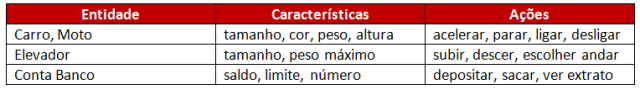
\includegraphics{abstracao.jpg}
                            \caption{\small Abstração do mundo real.}
                            \label{cap:conceitos}
                        \end{figure}
                \item \textbf{Classes}: Definição dada para a estrutura de um objeto, onde são definidas os atributos e métodos referentes a cada objeto.
                \item \textbf{Objetos}: É a instância de uma classe. Um objeto é a construção de software que encapsula estado e comportamento nos permitindo modelar a aplicação em termos reais e abstrações.
                \item \textbf{Herança}: É a possibilidade de uma classe \emph{(subclasse)} herdar métodos e atributos de outra classe \emph{(superclasse)}
                        \begin{figure}[!htb]
                            \centering
                            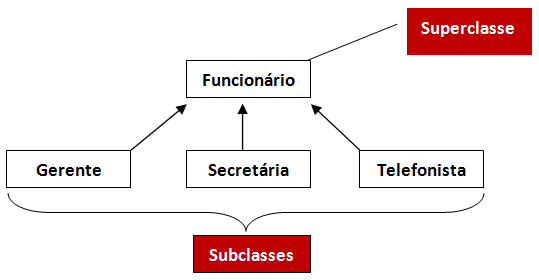
\includegraphics{heranca.jpg}
                            \caption{\small Hieraquia de classes}
                            \label{cap:heranca}
                        \end{figure}
                \item \textbf{Polimorfismo}: Se trata da capacidade de um método ou comportamento da \emph{superclass} ser implementado de diversas maneiras nas \emph{subclasses}.
                \item \textbf{Encapsulamento}: Forma de proteção dos atributos de uma classe, não permitindo que este seja acessado diretamente.

            \end{itemize}


    \section{MVC \emph{(Model, View e Controller)} \label{sec:mvc}}
        O MVC é um Design Pattern \emph{(Padrão de projeto)} utilizado para separar as camadas de modelo, visão e controle no desenvolvimento de um sistema. A camada de modelo \emph{(Model)} contém classes que implementam a regra de negócios da aplicação, já a camada de visão \emph{(View)}, por sua vez, são responsáveis pela exibição e apresentação dos dados para o usuário, e por fim a camada de controle \emph{(Controller)}, onde é processado todas as requisições realizadas pelo usuários.

        A separação da aplicação em camadas, como é feita no padrão MVC, trás uma série de vantagens no processo de desenvolvimento, uma delas é a de permitir a reutilização do mesmo objeto de modelo em visualizações distintas, além de organizar seu projeto de forma onde tudo tenha seu lugar, e cada camada com sua responsabilidade, permitindo um trabalho muitos mais "centrado" e modularizado.


    \section{CRUD \emph{(Create, Read, Update e Delete)}\label{sec:crud}}
        CRUD é o acrônimo da expressão do idioma inglês, \emph{Create Read Update and Delete} e é utilizado para designar as quarto operaçõs básicas de um banco de dados: Criar, Ler, Atualizar e Deletar.
        \begin{figure}[!htb]
            \centering
            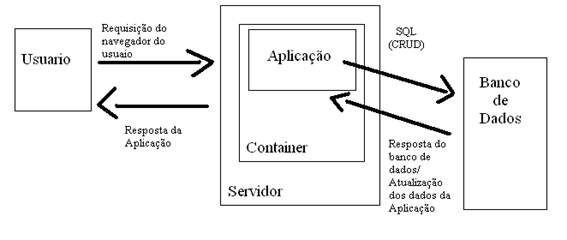
\includegraphics{crud.jpg}
            \caption{\small Execução de uma requisição CRUD}
            \label{cap:crud}
        \end{figure}

        Tratando como uma forma mais técnica o CRUD se transforma em um facilitador, criado através de diretivas de programação, para ações ligadas ao \emph{INSERT}, \emph{UPDATE}, \emph{DELETE} e \emph{SELECT} do banco de dados.



    \section{UML\label{sec:uml}}
        UML \emph{(Unified Modeling Language)}, é uma linguagem de modelagem possibilita o desenvolvimento de diagramas de classes, de objetos, casos de uso, entre outros. Esses diagramas são uteis para o desenvolvimento e um grande facilitador para o entendimento de um projeto e sua estrutura.

        \begin{figure}[!htb]
            \centering
            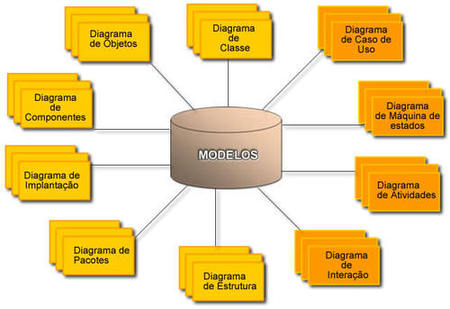
\includegraphics{uml.jpg}
            \caption{\small Exemplo de um diagrama UML.}
            \label{cap:uml}
        \end{figure}


    \section{Mysql\label{sec:mysql}}
        O MySQL é um gerenciador de banco de dados de código aberto, capaz de atender às necessidades dos mais variados tipos de usuários. Este produto tem uma gama diversificada de possibilidades de uso, algumas delas são soluções em desenvolvimento de sistemas, provedores, aplicações livres entre outras.

    \section{PDO\label{sec:pdo}}
        PDO \emph{(PHP Data Objects)} é um módulo de PHP montado sob o paradigma Orientado a Objetos e cujo objetivo é prover uma padronização da forma com que PHP se comunica com um banco de dados relacional. Este módulo surgiu a partir da versão 5 de PHP. PDO, portanto, é uma interface que define um conjunto de classes e a assinatura dos métodos de comunicação com uma base de dados. (LOCAWEB, 2015)

    \section{HTML\label{sec:hmtl}}
        HTML \emph{(Hyper Text Markup Language)}, como o próprio nome já diz, trata-se de uma linguagem de marcação de hipertexto utilizada no desenvolvimento de páginas web. Ela nos possibilita estruturar uma página através de marcações e tags específicas permitindo que a mesma seja acessada pela internet.

    \section{Node.js\label{sec:node-js}}
        \emph{Node.js} é uma plataforma constuida sobre o motor de Javascript que tem como principal objetivo fornecer uma maneira fácil de se construir programas de rede escaláveis. Mesmo sendo um servidor de programas não podemos confundi-lo com um servidor \emph{ready-to-install}(prontos para instalar), que são servidores que estão prontos para instalar aplicativos instantâneamente. O \emph{Node.js} segue o conceito de módulos que podem ser adicionados em seu núcleo. Há literalmente centenas de módulos para rodarem com o Node, e a comunidade é bastante ativa em produzir, publicar e atualizar dezenas de módulos por dia.

    \section{Automatizador Grunt\label{sec:automatizador-grunt}}
        \emph{Grunt} é uma ferramenta que roda via termina e serve para automatizar tarefas de uma aplicação,  como: concatenação, minificação e validação de arquivos, otimização de imagem, testes unitários, deploy de arquivos por ftp ou rsync, entre outras. O \emph{Grunt} é feito totalmente em \emph{Javascript} e roda no \emph{Node.js}, portanto para ser utilizado, depende da instalação do \emph{Node.js} e do pacote \emph{NPM} previamente instalados.

    \section{Sass\label{sec:sass}}
        É um pre-processador de folhas de estilo feito em \emph{Ruby} e responsável em auxiliar na produtividade de códigos \emph{CSS}. Literalmente falando, \emph{Sass} é uma extensão do \emph{CSS} que adiciona potência e elegância à linguagem básica. Ele permite ao desenvolvedor o uso de variáveis, mixins, importações, ampla organização do código, entre outras funcionalidade totalmentes compatíveis com \emph{CSS}. \emph{Sass} trabalha com dois tipos de \emph{sintax} diferentes, \emph{.sass} e \emph{.scss} e suas particularidas são: enquanto no arquivo \emph{.scss} são utilizados chaves \emph{"\{\}"} e ponto e vírgula \emph{";"} para delimitar o inicio e fim de atributos e valores, no \emph{.sass} essa delimitação é feita apenas por identação. Para ser utilizado em uma aplicação em produção utilizamos o arquivo \emph{CSS} gerado através da compilação do arquivo \emph{.sass} ou \emph{.scss}.

        \begin{figure}[!htb]
            \centering
            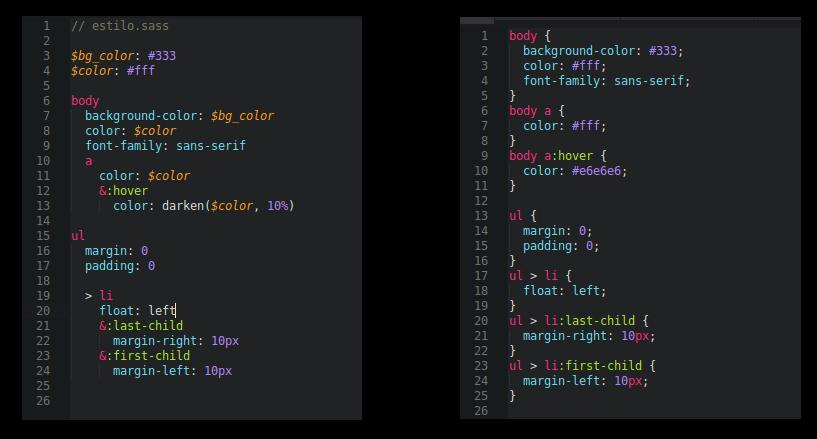
\includegraphics[scale=0.9]{sass.jpg}
            \caption{\small Compilação de um arquivo sass para css}
            \label{cap:sass}
        \end{figure}


    \section{Uglify\label{sec:uglify}}
        É um modulo que funciona em \emph{NodeJs} responsável pela minificação e compressão de arquivos \emph{Javascript}. Minificação consiste em reduzir o código, deixando-o apenas com o que é necessários para seu funcionamento, sem afetar nenhuma funcionalidade.


    \section{Rsync\label{sec:rsync}}
        \emph{Rsync} é uma ferramente que funciona apenas em sistemas \emph{Unix}, responsável por transferência de arquivos e capaz de sincronizar diretórios tanto locais quanto remotos. O \emph{Rsync} pode transferir arquivo \emph{Local -> Local}, \emph{Local -> Remoto}, \emph{Remoto -> Remoto}, \emph{Remoto -> Local}. Ele trabalha sobre o protocolo SSH e \emph{remote-update}, o que aumenta consideravelmente a velocidade e diminui a quantidade de dados transferidos, pois são trocados entre os servidores somente as diferenças entre dois grupos de arquivos reduzindo, também, o consumo de banda, além de ser muito mais seguro.


    \section{Controle de Versão: Git\label{sec:git}}
        É um sistema de controle de versão distribuído e open source que registra as mudanças feitas em um ou mais arquivos de forma que você possa recuperar versões específicas. Ele nos permite reverter arquivos ou até projetos inteiros para um estado anterior, comparar mudanças feitas com o tempo, ver qual desenvolvedor alterou determinado arquivo que pode estar causando problemas, entender em que ponto do projeto surigu determinada falha no sistema entre outras funcionalidades.

    \section{Github\label{sec:github}}
        \emph{Github} é um repositório online que utiliza o \emph{Git} como controle de versão e armazena diversos projetos, facilitando em processos de instalação e permitindo colaboração de outros desenvolvedores.


    \section{Bootstrap\label{sec:bootstrap}}
        É um framework de front-end que tem o objetivo de facilitar o desenvolvimento de interfaces para web. Contém uma coleção de vários elementos e funções personalizáveis para projetos da web, empacotados previamente em uma única ferramenta. Por se tratar de um software livre, todos os seus elementos são personalizaveis e utilizam uma combinação de HTML, CSS e Javascript.

    \section{Javascript\label{sec:javascript}}
        É uma linguagem de programação \emph{client-side} utilizada para controlar \emph{HTML} e \emph{CSS} manipulando comportamentos e elementos de páginas web.


    \section{Jquery\label{sec:jquery}}
        É uma biblioteca que tem como objetivo simplificar tarefas complexas da programação em \emph{Javascript}. Sua intenção é que fazer com que o desenvolvedor codifique menos porém tenha o mesmo, ou um melhor resultado sobre determinada ação.

        Entre as suas características principais, a biblioteca jQuery contém:

        \begin{itemize}
            \item Manipulação do HTML/DOM;
            \item Manipulação CSS;
            \item Métodos de eventos HTML;
            \item Efeitos e animações;
            \item (\emph{AJAX}) Ferramenta Jquery para trocar de informações com servidor sem precisar atualizar a página web atual;
            \item Entre outras funcionalidades genéricas.
        \end{itemize}
